\section{Περιγραφή πειραμάτων}

\subsection{Γενική περιγραφή των πειραμάτων}

Τα πειράματα πραγματοποιήθηκαν σε κρεβατοκάμαρα σπίτιου,στο δωμάτιο που φαίνεται στην εικόνα \autoref{fig:room}.
Το δωμάτιο φαίνεται στην εικόνα,και θα το περιγράφουμε και εμείς έτσι,όπως το βλέπει κάποιος που μπαίνει από την πόρτα και κοιτάει το δωμάτιο.
Θα μιλήσουμε σε σχέση με αποστάσεις από κοντινότερους τοίχους,καθώς είναι πολύ δύσκολο να έχεις υπόψη σου που βρίσκεται πάντα το νοητό
κέντρο του δωματίου.
Γενικά,θα θεωρήσουμε σαν αρχικές πλευρές τις πλευρές της γωνίας που βρίσκεται η πόρτα,δηλαδή από τον κάτω και δεξιό τοίχο,
και σαν τελικές πλευρές τον πάνω και αριστερό τοίχο.

Οι διαστάσεις τους δωματίου είναι 4 μέτρα μεταξύ του μπροστινού και πίσω τοίχου,
που ονομάζουμε \textbf{μήκος δωματίου} ή \textbf{y axis},δηλαδή άξονας Υ,
και 3.25 μέτρα μεταξύ του δεξιού και αριστερού τοίχου,
που ονομάζουμε \textbf{πλάτος δωματίου} ή \textbf{x axis},δηλαδή άξονας X.

Για τον \textbf{y axis},ο πίσω τοίχος είναι το \textbf{y axis=0} και ο μπροστά τοίχος είναι το \textbf{y axis=4}.
Για τον \textbf{x axis},ο αριστερός τοίχος είναι το \textbf{x axis=0} και ο αριστερός τοίχος είναι το \textbf{x axis=-3.25}.
Ο λόγος που επιλέχθηκε να ανεβαίνει θετικά ο άξονας Υ και να ανεβαίνει αρνητικά ο άξονας X,
είναι γιατί μπορούμε να σχεδιάσουμε το δωμάτιο σαν να σχεδιάζουμε στο δεύτερο τερτατημόριο ενός καρτεσιανού συστήματος. 


Έτσι όπως φαίνεται το δωμάτιο από την εικόνα,υπάρχει ένα παράθυρο στο πάνω τοίχο και μία μπαλκονόπορτα στο κάτω τοίχο.
Οπότε το δωμάτιο μπορούσε να αεριστεί πολύ εύκολα και γρήγορα.
Η πόρτα που βρίσκεστε στην κάτω δεξία γωνία,ανοίγει σε δωμάτιο που δεν έχει κάποιο ανοιχτο δωμάτιο,
οπότε στα πειράματα που η πόρτα ήταν ανοιχτή,δεν υπήρχε τόσο άμεση επαφή με τον εξωτερικό χώρο,για να είναι σαν έχουμε ανοιχτό παράθυρο.
Ωστόσο,ο αέρος που ερχόταν από άλλα δωμάτιο πρόσθετε πιο πολλές παραμέτρους που χρειάζεται να λάβουμε υπόψη,οπότε στα περισσότερο 
πειράματα που συμπεριλαμβάνουμε στα πειράματα,η πόρτα είναι κληστή.

\begin{figure}[!htbp]
    \centering
    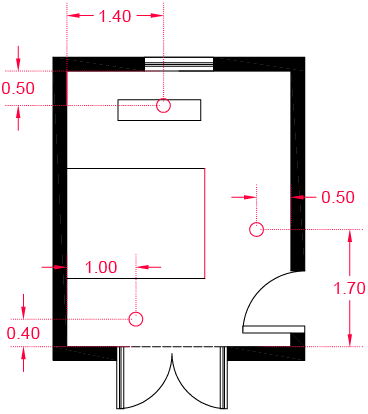
\includegraphics[width=0.8\textwidth]{εικόνες/εικόνες σχετικά με τον server/δωμάτιο διαστάσεις.png}
    \caption{Δωμάτιο που έγιναν τα πειράματα}
    \label{fig:room}
\end{figure}

Τα κύρια έπιπλα που υπάρχουν στο δωμάτιο είναι το κρεβάτι,που είναι κεντρικά και κολλημένα στον αριστερό τοίχο,
και μία κοντή σε ύψος βιβλιοθήκη,οπού βρίσκεται στο πάνω μέρος του δωματίου,που μπορεί να θεωρηθεί ότι είναι ένα είδος γραφείου.
Υπάρχει ένας ανεμιστήρας στο ταβάνι του δωματίου,ο οποίος χρησιμοποιήθηκε για κάποια πειράματα,
αλλά δεν χρησιμοποήθηκε για τα πειράματα που αναλύουμε.
Παρόλα αυτά,αξίζει να αναφερούμε ότι ένας ανεμιστήρας με κλειστή την μπαλκονόπαρτα 
και το παράθυρα έκανες τους αισθητήρες να δίνουν πολύ πιο γρήγορα απαντήσεις.


οι συσκευές τοποθετήθηκαν σταθερές στα σημεία που φαίνονται στην εικόνα του δωματίου,3 μικροελεκτές esp32 με αισθητήρες bme680.
Ο διαχωρισμός των συσκευών μπόρεσε να γίνει λόγω των διαφορετικών breadboard που είχε η κάθε συσκευή. 
Αυτό είναι πολύ σημαντικό, γιατί οι συσκευές χρειαζόταν να μετακινώνται,όταν ήταν απενεργοποιημένες για την ασφάλεια τους.
Δίναμε ρεύμα στις συσκευές αυτές μέσω καλωδίου σε μπρίζα και όχι με μπαταρία ή κάποιου είδους εσωτερική παραγωγή ενέργειας,
ωστέ να μπορούν να μένουν σταθερά στην ίδια θέση χωρίς μεγάλο πρόβλημα.
Επίσης,οι θέσεις στις οποίες βάζαμε τα έπιπλα κατά την διάρκεια των πειραμάτων,
δεν θα μπορούσε να διατηρηθεί έτσι κατά την κανονική χρήση του δωματίου.

Οι θέσεις των συσκευών και των σημείων που τοποθετούμε την πηγή ρύπου,περιγράφεται σε σχέση με τους δύο πιο κοντινούς τοίχους.
Στο βασικό πειραμά μας ,η συσκευή με \textbf{Id=0} είναι μισό μέτρο από το μπροστά τοίχο και 1.4 μέτρα από τον αριστερό τοίχο,
η συσκευή  \textbf{Id=1} είναι μισό μέτρο από το δεξί τοίχο και 1.7 μέτρα από το πίσω τοίχο 
και η συσκευή \textbf{Id=2} είναι μισό μέτρο από τον πίσω τοίχο και 1 μέτρο από τον αριστερό τοίχο. 

Καθε συσκευή και σημείο πηγής βρίσκεται στο ίδιο ύψος,που ήταν τα 60 εκατοστά.
Στην βιβλιογραφία σημειώνεται ότι για την καλύτερη εικόνα της έκθεσης των ανθρώπων στους ρύπους του αέρα,πρέπει να έχεις τους αισθητήρες στο 
ύψος αναπνοής των ανθρώπων.
Οπότε το επιλεγμένο ύψος είναι χαμήλο υπό κανονικές περιπτώσεις, οπού άνθρωποι θα υπήρχαν στον χώρο,αλλά για τα συγκεκριμένα πειράματα 
δεν κρίνεται απαγορευτικό.
Επίσης κανένας από τους αισθητήρες δεν έχει έπιπλο ή τοίχο μεταξύ αυτού και όλων των πηγών ρύπων για τους οποίους συλλέξαμε πληροφορίες.

Έγιναν πολλά πειράματα κάτα την διάρκεια του καλοκαιριού,στα οποία έχουμε κρατήσει τα δεδομένα,
αλλά δεν θα συμπεριληφθούν στην μετέπειτα ανάλυση και εύρεση των μηχανικών μοντέλων.
Ο ένας λόγος που γίνεται αυτό είναι γιατί δοκιμάστηκαν διάφορες συνθήκες που να επικρατεί στο πείραμα,
όπως με ανεμιστήρα ή να υπάρχει άνθρωπος στο δωμάτιο,όπως και δεν είχαμε κατασταλάξει στην μορφή που θα έχει το πείραμα.

Ο δεύτερος λόγος είναι ότι χρειάστηκε να αλλάξουμε τους αισθητήρες,
επειδή κατά την διάρκεια των πειραμάτων,
ο αισθητήρας CCS811 σταμάτησε να δουλεύει και παρατηρήθηκε πρόβλημα στα bme680,συγκεκριμένα στην εγκατάσταση που είχε γίνει στα pin header,που συνδέουν το Adafruit breakout BME680 με το breadboard,ώστε να μπορεί μέσω καλωδίων να πάρει ρεύμα από τον NODEMCU32S development board και να στείλει δεδομένα.
Ευτυχώς,οι NODEMCU32S δεν χρειάστηκαν αλλαγή.

Η περιόδος πειραμάτων,στις οποίας θα πάρουμε τα δεδομένα για την δημιουργία των μοντέλων,πραγματοποιήθηκε σε διάστημα δύο εβδομάδων,από τις 10 Οκτώμβρη 2025 εώς 24 Οκτώμβρη 2025.
Οι θέσεις που επιλέχθηκαν είναι οι εξής 16 θέσεις που απεικονίζονται με μπλε τελίτσα στην εικόνα \ref{fig:roomSources}.Για κάθε θέση,πραγματοποιήθηκαν 6 πειράματα τουλάχισταν.

\begin{figure}[!htbp]
    \centering
    
\includegraphics[width=0.8\textwidth]{εικόνες/εικόνες σχετικά με τον server/plotted room.png}
    \caption{Σημεία που τοποθετήθηκε η πηγή ρύπου στον χώρο}
    \label{fig:roomSources}
\end{figure}

\FloatBarrier 


\subsection{Περί της πηγής ρύπου}

Η πήγη ρύπου VOC που επιλέξαμε να καταμετρήσουμε ήταν καθαρό αλκοόλ,περιεκτικότητας $95^\circ$ σε Αιθυλική αλκοόλη,δηλαδή εθανόλη.
Οι λόγοι που χρησιμοποιήσαμε καθαρό αλκοόλ είναι διότι αποτελεί ένα πολύ κοινό καταναλωτικό προίον,
που αποτελεί πηγή VOC ρύπων,δεν αποτελεί ιδιαιτερά επικύνδινο για την υγεία και εμπεριέχει εθανόλη,που ξέρουμε ότι είναι αέρια χημική ουσία πάνω στην οποία ο BME680 αισθητήρας αέρα έχει ελεγχθεί.

Σε κάθε πείραμα,φροντίζαμε να υπάρχουν 30 ml φαρμακευτικού αλκοόλ στο μπολάκι που χρησιμοποιήσαμε για τα πειράματα.
Το μπολάκι αυτό,ενώ ήταν στο μέγεθος που μπορούσε κάποιος άνετα να το κρατήσει σε μία παλάμι,
ήταν σχετικά βαθή για τα 30 ml που του βάζαμε μέσα,όποτε δεν ξέρουμε αν αυτό μείωνε την εξάτμιση που θα περιμέναμε να δούμε ή οχι. 
Αλλά χάρη στο βάθος του,δεν είχαμε προβλήματα του να χείνεται το αλκοόλ,σε αντίθεση με το 
αν χρησιμοποιούσαμε ένα αβαθές πιατάκι.

Δυστυχώς,δεν καταφέραμε να βρούμε εξίσωση για να υπολογίσουμε πόσα ppm εθανόλης εξατμιζόντουσαν ανά λεπτό,
ή πόσα ppm εθανόλης θα έπρεπε να περιμένουμε.
Δεν είναι παράξενο που δεν βρέθηκε μια γενική συνάρτηση,καθώς υπάρχουν πολλές περιβαλλοντογικές μετάβλητες που καθορίζουν την ταχύτητα εξάτμισης και 
δεν έχουμε καλή χημική γνώση για να το υπολογίζαμε εμείς.

Ακόμα,δεν ξέραμε κάθε φορά ,πόσα απο τα 30  ml ήταν νερό και πόσα εθανόλη,
διότι κρατούσαμε το αλκοόλ ανάμεσα από τα πειράματα.
Θα ήταν πολύ δαπάνειρο να χύνουμε κάθε φορά το αλκοόλ και να το συμπληρώναμε 30 ml,
αφού το καθαρό αλκόολ κοστίζει γύρω στο 10 εύρω για 100-200 ml.
Θα μπορούσαμε να χρησιμοποιήσουμε αλκοολούχα λοσιόν $70^\circ$,που για 240 ml βρίσκεις στα 1-1,5 ευρώ,
αλλά δεν ξέραμε αν θα μπορούσε να αναγνωρίσει ο αισθητήρας αέρα του BME680 τις άλλες χημικές ουσίες που έχει η εθανόλη, 
οπότε προτιμήσαμε το καθαρό αλκοόλ που έχει μεγαλύτερο ποσοστό εθανόλης,που είμαστε σίγουροι ότι ο BME680 θα αντιδράσει σε αυτές.
Κλείνουμε το μπολ με το αλκόολ σε κουτί κατά την διάρκεια.

\subsection{Τι εννοούμαι με πειράματα και  κύκλους πειραμάτων.Calibration των αισθητήρων}

Σαν ένα πείραμα,ονομάζουμε την περίοδο πριν και μετά την εισαγωγή της πηγής ρύπου στο δωμάτιο όπου λαμβάνουμε υπόψη τις τιμές των αισθητήρων, για την μετέπειτα ανάλυση τους και χρησιμοποίηση τους σε μηχανικά μοντέλα.

Η χρονική περίοδος που είναι πριν την εισαγωγή του ρύπου, την δηλώνουμε
σαν \texttt{experimentState=StartingExperiment}.
Από αυτήν την στιγμή και μετά λαμβάνουμε υπόψη τα δεδομένα.
Η χρονική περίοδος που είναι μετά την εισαγωγή του ρύπου, την δηλώνουμε σαν \texttt{experimentState = RemovingSourcePollutant}.
Από αυτήν την στιγμή και μετά σταματάμε να λαμβάνουμε υπόψη τα δεδομένα.
Ενδιάμεσα,δηλώνουμε ότι προκείται να εισαχθεί η πηγη σαν \texttt{experimentState=InsertingSourcePollutant} στο server.

Ένας κύκλος πειραμάτων περιλαμβάνει πολλά τέτοια πειράματα,που ξεκινάει από την στιγμή που βάζουμε τις συσκευές στην μπρίζα,
μέχρι την στιγμή που σταματάμε να κάνουμε άλλα πειράματα για την συγκεκριμένη μέρα.
Συνήθως αυτό σήμαινε ότι βγάζαμε τις συσκευές από την μπρίζα,για μεγαλύτερη ασφαλεία τους.

Ο λόγος που ορίζουμε σαν ένα κύκλο πειραμάτων με τέτοιο τρόπο είναι γιατί  αφού βάζουμε τις συσκευές στην πρίζα,
πρέπει να κάνουμε calibrate τους αισθητήρες κάθε φορά.
Η διαδικάσια calibration των αισθητήρων αέρα της bsec,συμφώνα με τις περιγραφές στα αρχεία της BSEC βιβλιοθήκη και στο αρχείο οδηγειών ενσωμάτωσης,
πρέπει να μείνει ο αισθητήρας να μείνει 30 λεπτά σε καθαρό αέρα και 30 λεπτά ρυπαρό αέρα.
Σαν παράδειγμα έκθεσης σε ρυπαρό αέρα,δίνεται το να βάλεις τον αισθητήρα σε ένα κουτί που εμπεριέχει
εκπνεόμενο από τον άνθρωπο αέρα.

Στην περίπτωση μας,τοποθετούμε το αλκοόλ μαζί με την συσκευή σε ένα κουτί,και το κλείνουμε όσο γίνεται με καπάκι.
Αυτό το κάνουμε όταν βλέπαμε στην grafana ότι στον πίνακα \textbf{Ακρίβεια},η τιμή  \texttt{accuracy}(ακρίβεια)  από το 0 έχει φτάσει στο 1 και έχει παραμείνει εκεί για κάποια λεπτά,για τον αισθητήρα της συσκευής με ένα δεδομένο \textbf{Id}.
Ο λόγος που δεν βάζαμε την συσκευή από το κουτί από την  αρχή είναι ότι όταν ο αισθητήρας βρίσκεται σε \texttt{accuracy=0}, 
υπάρχει ακόμα μία διαδικασία σταθεροποίησης της BSEC λογισμικού, όπως φαίνεται από τις μεταβλητές \texttt{\detokenize{BSEC_OUTPUT_STABILIZATION_STATUS}} και \texttt{\detokenize{BSEC_OUTPUT_RUN_IN_STATUS}}.
Και ο ίδιος ο οδηγός ενσωμάτωσης μας συμβουλεύει να αρχίσουμε το calibration όταν η ακρίβεια έχει φτάσει στο 1

Δεν υπήρχε πρόβλημα να αφήσουμε τον BME680 σε καθαρό αέρα για 30 λεπτά,γιατί με ανοιχτά παράθυρα,αυτή η προυπόθεση εκπληρωνόταν πολύ εύκολα.
Δυστυχώς,αυτό δεν ήταν τόσο εύκολο να το εκπληρώσουμε για την έκθεση σε ρυπαρό αέρα να το εκπληρώσουμε,
γιατί είχαμε μόνο ένα μπολ πηγής πυο χρησιμοποιούσαμε και υπήρχε κίνδυνος αναποδογυρίσματος του κουτιού,
σε περίπτωση που βάζαμε και τις 3 συσκευές μες το κουτί.
Επείδη κάναμε την διαδικάσια την παραπάνω μία συσκευή την φορά,αν το αφήναμε μίση ώρα μες το κουτί κάθε συσκευη,
η παραπάνω διαδικασία θα έπαιρνε τουλάχιστον μιάμισή ώρα.

Οπότε αυτό που κάναμε ήταν ότι αφήναμε την συσκευή στο κουτί με τον αλκόολ,χωρίς να βραχεί ενοείται,μέχρι να δούμε ότι η ακρίβεια της συγκεκριμένης συσκευής 
έχει πάει στο 2 και έχει παραμείνει για κάποιο χρονικά διάστημα σε αυτή.
Το \texttt{accuracy=2} δεν υποδηλώνει την βελτιστή ποιότητα,αλλά σημαίνει ότι ο αισθητήρας μπορεί να προσεγγίσει μια τιμή VOC και επηρεάζεται ακόμα και στις μη ακραίες συνθήκες περιβάλλοντος.
Και έπειτα παρατηρήθηκε εμπειρικά,ότι η BSEC μπορεί να σταθεροποιηθεί η ίδια στη βέλτιστη ακρίβεια, αν και έχουμε αρκετές περιπτώσεις όπου η ακρίβεια πάει από το 2 στο 3,
χωρίς όμως να πέφτει πότε στο 1 ή στο 0,παραμόνο εάν κατέρεε ο server κατά την διάρκεια αποστολής δεδομένων.
Παρόλο που η παραπάνω διαδικάσια μείωνε τον χρόνο αναμονής του calibration, έπαιρνε τουλάχιστον μία ώρα.

Για την περίπτωση που θέλαμε να κάνουμε inter-calibration,δηλαδή να ρυθμίσουμε τους αισθητήρες ώστε να έχουν παρόμοια τιμή μεταξύ τους,κάναμε και πειράματα
όπου οι συσκεύες ήταν όλες μαζί.
Ένα πείραμα γινόταν χωρίς να υπάρχει η πηγή ρύπου στον χώρο και ένα ακόμα πείραμα με της ύπαρξη της πηγής ρύπου μες τον χώρο.
Αυτά τα παραπάνω γινόντουσαν μετά την διαδικασία calibration,ωστέ να ξέρουμε για την συνέχεια του κύκλου των πειραμάτων πόσο διαφοροποιούνται οι αισθητήρες στην ίδια θέση.

Αυτό που διαφοροποιεί κάπως την διαδικασία ενός πειράματος σε σχέση με ότι περιγράφτηκε παραπάνω είναι ότι για τα πειράματα χωρίς κάποια πηγή,
η πρώτη φάση δεν διαρκεί καθόλου χρόνο, αφού θα έχουμε συνεχίσει κατάσταση ηρεμίας έτσι και αλλιώς.
Πείραμα χωρίς κάποια εισαγωγή πηγής  

Δεν έχουμε πρόσβαση στην διαδικασία calibration της BSEC,οπότε δεν ξέρουμε αν οι διαφοροποιήσεις είναι λόγω μικρών κατασκευαστικών διαφορών στους αισθητήρες αέρα ή είναι διαφορετικά λόγω των εσωτερικών μοντέλων της BSEC.
Επίσης,τα μηχανικά μοντέλα τα εκπαιδεύσαμε στα δεδομένα του κάθε αισθητήρα ξεχωριστά,οπότε δεν χρειάστηκε να συμφωνούν οι αισθητήρες μεταξύ στο να έχουν παρόμοια δεδομένα τα ίδα ppm αέρα.
Αλλά είναι χρήσιμα δεδομένα για κάποια μελλοντική ανάλυση των δεδομένων.

Αφότου είχαν γίνει τα παραπάνω,ο στόχος για κάθε κύκλου πειραμάτων ήταν να τρέξουμε τουλάχιστον ένα πείραμα και για τις 16 θέσεις που είχαμε ορίσει.
Αλλά αυτό δεν ήταν πάντα εφικτό,γιατί κάθε πείραμα,όπως θα περιγραφεί στο επόμενο κομμάτι κείμενου,το ίδιο το πείραμα και η προετοιμασία έπαιρνε κάπου στα είκοσι λεπτά με μίση ώρα.
Ακόμα,σε περιπτώσεις που μπλοκαριζόταν η δειγματοληψία ενός αισθητήρα για αρκετά μεγάλο διάστημα,έπρεπε να ξανακάνουμε την διαδικάσια calibration,που οδηγούσε το κύκλο πειράματων σε ένα είδος μικρής επανεκίνησης.
  
Ο λόγος που επιλέχθηκαν τα συγκεκριμένα 16 σημεία είναι για να υπάρχει ισοροπημένη και πλήρη κάλυψη του δωματίου,με κάθε σημείο να ισαπέχει με το άλλο σχεδόν ένα μέτρο μεταξύ του άξονα Χ και του άξονα Υ.
Για τον άξονα Υ,αυτό ήταν εφικτό.
Όμως, το μέγεθος του δωματίου είναι 3.25 στο πλάτος,και δεν θέλαμε να κολήσουμε κάποια πηγή στον τοίχο,οπότε επιλέξαμε σαν τελική απόσταση από τον δεξί τοίχο το \textbf{x axis=-2.95}
\subsection{Αναλύτικη περιγραφή ενός πειράματος και πως φαίνεται στην ιστοσελίδα}


Στην εικόνα \ref{fig:defaultSite},φαίνεται η αρχική κατάσταση της ιστοσελίδας που αλλελπιδρά ο χρήστης.
Είναι φτιαγμένη με σκοπό να μην χρειάζονται ειδικές γνώσεις για να χειριστεί κάποιος την εφαρμογή.

Στο κάτω μέρος υπάρχει το κομμάτι που ο χρήστης δηλώνει υγρασία και θερμοκρασία,αλλά όπως αναφέρθηκε και προηγούμενης,δεν χρησιμοποιήθηκε στα προκειμένα πειράματα.
Δίνεται πρόσβαση στο url που κατευθείνει τον χρήστη στην grafana όπου υπάρχει η οπτικοποίηση σε ζωντανό χρόνο.
Επίσης,υπάρχει κομπί για μία περιγραφή της διαδικασίας του πειράματος και δυνατότητα να αποσταλούν τα σημερίνα log του server στον χρήστη.

\begin{figure}[!htbp]
    \centering
    \includegraphics[width=0.8\textwidth]{}
    \caption{Αρχική μορφή της ιστοσελίδας}
    \label{fig:defaultSite}
\end{figure}

Αφού ο χρήστης έχει κλείσει τα παράθυρα και την πόρτα και έχει περιμένει κάποια λεπτά, ώστε η τιμή VOC να αυξηθεί από την κατάσταση που το δωμάτια έχει ανοιχτά το παράθυρο και την μπαλκονόπορτα,
που θα αρχίζουμε να τα λέμε και τα δύο παράθυρα,γιατί και τα δύο επιτελούν τον ρόλο του να αερίζουν το δωμάτιο με εξωτερικό αέρα.

Αφού παρατηρηθεί από την grafana ότι οι τιμές VOC έχουν σταθεροποιηθεί σχετικά,δηλώνει ότι θέλει να ξεκινήσει καινούργιο πείραμα,πατώντας το κουμπί \textbf{Ξεκίνα καινούργιο πείραμα}.
Ο server αποθηκεύει στο collection  \texttt{UserInput} της βάσης δεδομένων,document με \texttt{userInputCategory="ExperimentState"} και \texttt{uexperimentState="StartingExperiment"} και την χρονική στιγμή της αποθήκευσης του document.
Έπειτα εμφανίζεται η παρακάτω μορφή της ιστοσέλίδας \ref{fig:afterInsertingStart}. 


\begin{figure}[!htbp]
    \centering
    \includegraphics[width=0.8\textwidth]{}
    \caption{Η ιστοσελίδα αφού έχει ξεκίνησει πείραμα}
    \label{fig:afterInsertingStart}
\end{figure}

Αφού περιμένουμε τουλάχιστον 1 με 2 λεπτά,για να υπάρχει περιθώριο δεδομένων ο χρήστης πατάει το κουμπί \textbf{},
για να προχωρήσει στην σελίδα που φαίνεται στην εικόνα \ref{fig:InsertingSourcePollutantDetails}.

\begin{figure}[!htbp]
    \centering
    \includegraphics[width=0.8\textwidth]{}
    \caption{Η σελίδα που δηλώνονται οι λεπτομέρειες του πειράματος}
    \label{fig:InsertingSourcePollutantDetails}
\end{figure}

\FloatBarrier 


\subsubsection{Λεπτομέρειες τις σελίδας εισαγωγής πηγής ρύπων }




\paragraph{Τύπος Ρύπου,Αντικείμενο προέλευσης,ποσότητα που χρησιμοποείται}

\paragraph{Δωμάτιο}

\paragraph{Θέση πηγής ρύπου}

\paragraph{Συνθήκες του δωματίο που ισχύουν}

\begin{itemize}
  \item
  \item 
  \item 
\end{itemize}
\subsubsection{Εισαγωγή πηγής ρύπου}

\begin{figure}[!htbp]
    \centering
    \includegraphics[width=0.8\textwidth]{}
    \caption{Η σελίδα αφότου δηλώθηκε η είσοδος πηγής ρήπου}
    \label{fig:sourcePollutantInserted}
\end{figure}


\FloatBarrier 
